\documentclass[a4paper,12pt, fleqn]{article}
\usepackage{multicol}
\usepackage{dirtree}
\usepackage[pdftex,colorlinks, citecolor=black, linkcolor=black, urlcolor=blue]{hyperref}
\usepackage[pdftex]{graphicx}
\usepackage{comment}
\usepackage{czt}
\usepackage{subfig}
\usepackage{longtable}
\usepackage[svgnames]{xcolor}
\usepackage[cm]{fullpage}

\renewenvironment{theorem}[2]{\vspace{3mm} {\bf Elimination Theorem} #1 [$#2$] \vspace{-3mm}\begin{zed}}{\end{zed}\vspace{-5mm}}

\renewcommand{\const}{\textrm{const }}
\newcommand{\sw}{\textrm{somewhere}}
\newcommand{\anything}{\textrm{anything}}
\newcommand{\eval}{\textrm{eval}}
\newcommand{\se}{\textrm{setExtension}}

\begin{document}

\thispagestyle{empty}

\begin{center}

\mbox{}\vspace{7cm}

{\Huge The Fastest 1.3.6 User's Guide}

\vspace{.5cm}

{\LARGE Automating Software Testing}

\vspace{2cm}

{\large Maximiliano Cristi\'{a}

{\tt mcristia@flowgate.net}

\vspace{0.5cm}


\begin{multicols}{2}
Pablo Rodr\'{\i}guez Monetti 

{\tt prodriguez@flowgate.net}

\vspace{0.5cm}

Pablo Albertengo

{\tt palbertengo@flowgate.net}

\end{multicols}}

\vspace{1.5cm}
\includegraphics[scale=.4]{logo.jpg}
\vspace{1.5cm}

{\large Flowgate Consulting 

Maip\'{u} 778 Piso 1 Oficina 10

(2000) Rosario

Argentina}

\vspace{1cm}

Release date: July 2010
\end{center}

\pagebreak

\tableofcontents

\pagebreak

\section{What's New on This Version}

\begin{itemize}
\item Command \verb+loadelimtheorems+ has been added.

\item In elimination theorems, set extensions can be better expressed through the directive \verb+\se+.

%AVISAR: si el conjunto por extensión de la clase de prueba tiene como uno de sus elementos un conjunto por comprensión (ver si esto lo acepta CZT), entonces prunett no va a podar esa clase.
%Los valores del conjunto no tienen que tener comas ",". Esta pensado para valores de tipos simples.

\item The general pruning algorithm was slightly changed (see section \ref{prunett}).

%AVISAR: Poda los nodos de los cuales podo todos los hijos, poda las hojas que no tienen caso de prueba, se puede volver a ejecutar prunett luego de genalltca.

\item The elimination theorem library delivered with this version is included in Appendix \ref{etl}.

\item This version partially supports axiomatic definitions (see section \ref{axdef}).
%AVISAR:
%setaxdef se debe ejecutar luego de loadspec y antes de prunett; antes de prunett se pueden cambiar valores, luego ya no se puede. 

\item Commands \verb+setaxdef+, \verb+showaxdef+ and \verb+showaxdefvalues+ have been added.

\item Limited support for four new testing tactics have been added: Numeric Ranges (NR), Mandatory Test Set (MTS), Weak Existential Quantifier (WEQ) and Strong Existential Quantifier (SEQ) (see sections \ref{nr}, \ref{mts}, \ref{weq} and \ref{seq}, respectively).

\item Testing tactics ISE, PSSE and SSE have been fixed to support expressions at the left of $\in$, $\subset$ or $\subseteq$, and not only variables.

\item Section \ref{tips} was added to document some tips on how to write Z models more suitable to be loaded on Fastest.

\item Appendix \ref{unsfeatures} lists some Z features {\it still} unsupported by Fastest.

\item An application-level parameter has been added to limit the number of evaluations when searching for abstract test cases (see section \ref{genalltca}).

\item It is possible to load specifications where terms are used before their declarations.

\item Command-line editing features (like tab completion) have been added (see section \ref{readline}).

%\item Command \verb+eval+ has been added to allow users to find values satisfying predicates (see section \ref{eval}).
\end{itemize}


 \pagebreak

\section{Introduction to Model-Based Testing}

\begin{itemize}
\item Testing could be the most costly phase of a software development project.

\item We can use formal methods to make testing almost automatic, thus changing the cost of testing by the cost of formalization---which is reported to be quite less expensive.

\item Model-based testing (MBT) uses a formal specification to generate test cases and to verify whether they found errors in the program or not.

\item Figure \ref{f:mbt} depicts one of the possible MBT methodologies, a part of which is implemented by Fastest. The methodology is based on \cite{Stocks2}, \cite{Horcher} and \cite{Stocks}.

\item Testing starts by writing a model of the software under test.

\item At the beginning, the model is used to generate test cases.

\item At the end, the model is used as an oracle.

\item The process is very automatic if we have the model.

\item The current version of Fastest only implements the {\it generation} phase of Figure \ref{method}.

\item Fastest is more suitable for unit testing.

\item {\bf The MBT methodology implemented by Fastest, called Test Template Framework (see next section), uses Z formal specifications.}
\end{itemize}

\begin{figure}[h]
\begin{center}
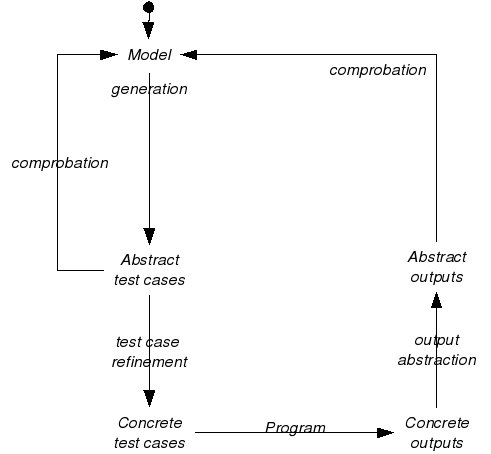
\includegraphics[scale=.9]{testing-func-01.png} 
\caption{\label{f:mbt}Model-based testing methodology: general view.}
\end{center}
\end{figure}







 \pagebreak

\input{ttf} \pagebreak

\input{arch} \pagebreak

\input{example} \pagebreak

\input{tips} \pagebreak

\section{\label{um}User's Manual}

Throughout of this manual remember that Fastest is still a prototype. Then, it is not as robust as it should be.

For an academic presentation of Fastest see \cite{CristiaPRM} and \cite{CristiaARM}.

\subsection{\label{ief}Installing and Executing Fastest}

Fastest should work on any environment with Java SE Runtime Environment 1.6 or newer. However, it has been tested only on Linux and MS-Windows boxes. To install the tool, just decompress and unarchive the file Fastest.tar.gz in any folder of your choice. 

Fastest can run in one of two modes, we call them \textit{application mode} and \textit{distributed mode}. Roughly speaking, in application mode all the processing is performed in the local computer, while in distributed mode some tasks can be distributed across so called {\it testing server}. In this section we explain how to run Fastest in application mode; section \ref{idts} explains how to run it as a distributed system. It should be noted that, although application mode is the easiest way to use Fastest and it provides the same functionality than in distributed mode, Fastest achieves all of its efficiency in distributed mode. 

\subsubsection{\label{readline}Running Fastest and Entering Commands}
To run Fastest in application mode, open a command window and run one of the following commands, where \verb+INSTALLDIR+ is the full path to the directory where Fastest was installed.

\begin{verbatim}
java -jar INSTALLDIR/fastest.jar

java -Xss8M -Xms512m -Xmx512m -jar INSTALLDIR/fastest.jar
\end{verbatim}

The first command will serve for most purposes, but if large specifications will be used then the second command is a better option. If the computer has at least 1 Gb of memory then the second option should be used. The \verb+Xms+ and \verb+Xmx+ options indicate the minimum and maximum amounts of memory that the Java process will be able to use, respectively. Then, if more memory is needed increase the maximum (it must be a multiple of 1024). In this version of Fastest it is difficult to know if more memory is needed, but one symptom is command \verb+genalltt+ (section \ref{genalltt}) taking too long---more than one minute---to finish.

In either case, Fastest prints the following prompt from which users can issue commands. 

\begin{verbatim}
Fastest>
\end{verbatim}

To enter a command just type-in it along with its arguments and then press the return key. There are three ways of learning which commands are available:

\begin{itemize}
\item Type \verb+help+ and press the return key.

\item Press the TAB key and a list of commands will be printed.

\item Type-in the first letters of a command and then press the TAB key: either a list of the commands whose name starts with those letters will be printed, or the complete command name, if any, will be printed. For instance, if after entering the \verb+a+ key the TAB key is pressed the following is printed (\verb+[TAB]+ means pressing the TAB key):

\begin{verbatim}
Fastest>a[TAB]

addtactic apply
Fastest>a
\end{verbatim}

And if the \verb+d+ key is pressed followed by the TAB key again, the result is the whole \verb+addtactic+ command printed, as follows:

\begin{verbatim}
Fastest>ad[TAB]dtactic 
\end{verbatim}
\end{itemize}

When the TAB key is pressed after command \verb+loadspec+, Fastest prints the contents of the working directory. For example, if Fastest is run from the installation directory, the result is as follows:

\begin{verbatim}
Fastest>loadspec [TAB]

doc                   fastest-server.jar    fastest.jar
lib
Fastest>showsch
\end{verbatim}

If the user types-in the first letters of one these files or directories and then presses the TAB key again, the name will be completed or a filtered list will be displayed, as with command names. If the letters correspond to a file name and it is completed, a blank space is added at the end; but if the letters correspond to a directory, when the name is completed a \verb+/+ or \verb+\+ character is added at the end. If the user presses the TAB key again, the content of this directory is displayed. The TAB key can be further pressed as a means of exploring the contents of the inner directories.

The left and right arrow keys can be used to move the cursor along the line being edited to modify it by inserting or deleting any character. The up and down arrow keys move across the commands that have been issued during the session. If one of these commands is recovered the user can modify it by using the left and right arrow keys, and can run it again by pressing the return key. Commands are executed when the return key is pressed regardless of where the cursor is.

\vspace{5mm}\noindent {\bf Important!!} Note that \verb!Ctrl+C! kills the program making all the data and commands to be lost. Future versions will be more robust.

\vspace{5mm}\noindent {\bf Important!!} Fastest does not save anything by default. The user has to use one of the commands described in section \ref{esr} to save the data generated during a session.

\subsection{Steps of a Testing Campaign}

Roughly speaking, currently, a typical testing campaign carried on with Fastest can be decomposed in the steps listed below. Some of them are optional and some can be executed in a different order, as is described in the referred sections between brackets. Also, at any time users can run commands to explore the specification and the testing trees, and to save their results (\ref{esr}). 

\begin{enumerate}
%\setcounter{enumi}{-1}
\item Install and declare more testing servers---i.e. run Fastest in distributed mode (\ref{idts}).

\item\label{s:loadspec} Load the specification (\ref{leso}).

\item\label{s:selop} Select the operations to be tested (\ref{leso}).

\item\label{s:addtactic} Select a list of testing tactics to be applied to each operation (\ref{tactics}).

\item\label{s:genalltt} Generate testing trees (one for each selected operation) (\ref{genalltt}).

\item\label{s:setaxdef} Set a value for each axiomatic definition (\ref{setaxdef}).

\item\label{s:prunett} Prune the trees (\ref{prunett}).

\item\label{s:genalltca} Calculate abstract test cases (\ref{genalltca}).

\item If some leaves do not have an abstract test case, then explore these leaves to determine the cause for that. There are two possible causes:

\begin{itemize}
\item The leaf predicate is a contradiction, but Fastest failed in pruning it. In this case:

\begin{enumerate}
\item\label{ietl} Improve the elimination theorem library with as many elimination theorems as necessary to prune all the contradicting leaves (\ref{elimtheor}).

\item Reload the elimination theorem library (\ref{let}).

\item Prune the trees again (\ref{prunett}).

\item Check whether all of the contradicting leaves have been pruned. If not, check the elimination theorems that were added and go to step \ref{ietl}.
\end{enumerate}

\item The leaf predicate is not a contradiction, but Fastest was not smart enough to find an abstract test case for it. In this case: 
\begin{enumerate}
\item Help Fastest to generate finite models to find abstract test cases for these complex test classes (\ref{setfinitemodel}).

\item Go to step \ref{s:genalltca}.
\end{enumerate}
\end{itemize}

\item If all of the leaves have an abstract test case, then save the results (\ref{esr}) and leave the program (\ref{quit}).
\end{enumerate} 

Step \ref{s:addtactic} is perhaps the most relevant step of all since it will determine how revealing and leafy testing trees are going to be. Along the same lines, step \ref{s:prunett} is highly recommended since it will severely reduce the time of most testing campaigns.

Test case design includes from step \ref{s:loadspec} to step \ref{s:genalltt}. The remaining steps generate test data, i.e. abstract test cases.

Note that once testing trees have been generated it is impossible to add more tactics.

The following sections explain in detail each of the steps of a testing campaign carried on with Fastest.


\subsection{\label{idts}Installing and Declaring Testing Servers}

We have mentioned earlier that Fastest, by definition, is a distributed system making it possible to parallelize testing tree pruning and the calculation of abstract test cases, between all the available servers. Hence, a typical Fastest facility would consist of some clients, used by test engineers to conduct the testing, and many servers, used by those clients, to prune testing trees and calculate abstract test cases --it is important to remark that servers need not to be powerful computers, in fact we think of them being custom workstations which are usually underutilized. If test engineers use Fastest wisely then, they can take advantage of the servers during idle hours, optimizing the computing power of the organization.

In this version, testing servers need to be declared in each computer running a client. The configuration file named \verb+lib/conf/cserversinfo.conf+ is a text file that stores the list of available testing servers --for that particular client. The syntax is as follows: 

\begin{verbatim}
name address port
\end{verbatim}

\noindent where, \verb+name+ is a descriptive name for the server (it has no use in this version), \verb+address+ is the IP address of the server, and \verb+port+ is the port number at which the server is listening to.

On the other hand, each server has to be started either manually with the command \verb+java -jar+ \verb+fastest-server.jar+; or it can be run by an operating system initialization script executing the same command. The port number where each server will listen for connections is declared in the configuration file \verb+lib/conf/server-port.conf+ by simply writing the number. Note that this number and the port number declared in the clients must coincide.

Fastest's default configuration is to run a client and a sever in the same computer. This is highly advisable since the client will be idle most of the time during a testing campaign. In the default configuration, client and server communicates through port 5001 while the IP address of the server must be 127.0.0.1.
 

\subsection{\label{leso}Loading a Specification and Selecting Operations}

An specification is loaded by executing \verb+loadspec+ followed by a file name. The full path to the file must be written if it is not located in the directory from which Fastest was started, as in the following example:

\begin{verbatim}
Fastest> loadspec doc/sensors-simp.tex
\end{verbatim}

It is assumed that the file is a text file containing the full specification; the current version does not support the \LaTeX{} directive \verb+\input{}+. If the specification contains syntactic or type errors it will not be loaded and the errors will be informed. It is possible to load only one specification at a time. To load a new specification run the \verb+loadspec+ command again or reset the current session by running command \verb+reset+ (in either case all the data generated so far will be lost). 

It is possible to load specifications where terms are used before their declarations.

Once a specification has been loaded, it can be explored, printed and saved with the commands described in section \ref{esr}.

After loading a specification the user has to select one or more operations to be tested. To do that use \verb+selop+ followed by the name of a Z schema representing an operation. The list of candidate Z schemas can be displayed with \verb+showloadedops+, with no arguments. It can be selected as many operations as needed by issuing the same number of \verb+selop+ commands. An operation that was previously selected can be deselected with command \verb+deselop+ followed by the name of the operation.


\subsection{\label{tactics}Selecting and Defining Testing Tactics}

The command \verb+addtactic+ adds a testing tactic to the list of tactics to be applied to a particular (previously selected) operation. Tactics are applied in the order they are entered by the user. Each tactic is applied to all the test classes of the current level of the testing tree, thus partitioning each of them according to the tactic's definition\footnote{This is a deviation from the original formulation of the TTF since according to it, a tactic has to be applied just to a given test class. Future versions of Fastest will work as suggested by the TTF.}. Initially, the list of tactics of any operation includes only the tactic named Disjunctive Normal Form (see below), which is the first to be applied.

The command syntax is rather complex because it depends on the tactic that is going to be applied (see the following sections for more details). The base syntax is: 

\begin{verbatim}
addtactic op_name tactic_name parameters
\end{verbatim}

\noindent where \verb+op_name+ is the name of a selected (Z) operation, \verb+tactic_name+ is the name of a tactic supported by Fastest, and \verb+parameters+ is a list of parameters that depends on the tactic. Unless the command prints an error message, the tactic has been successfully added. This command produces no other effect than adding the tactic to an internal list until command \verb+genalltt+ is executed (see section \ref{genalltt}).

Command \verb+showtactics+ prints a brief description of the available tactics; the following sections describe them in more detail.

\subsubsection{Disjunctive Normal Form}
This tactic is applied by default and it must not be selected with \verb+addtactic+. By applying this tactic the operation is written in Disjunctive Normal Form and the $VIS$ is divided in as many test classes as terms are in the resulting operation's predicate. The characteristic predicate of  each class is the precondition of one of the terms in the operation's predicate.

\subsubsection{Standard Partition (Fastest's name SP)}
This tactic uses a predefined partition of some mathematical operator (see ``Standard domains for Z operators'' at page 165 of Stocks' PhD thesis \cite{Stocks}). 

Take a look at Appendix \ref{sp} and at the file \verb+INSTALLDIR/lib/conf/stdpartition.spf+ to see what standard partitions are delivered with Fastest and how to define new ones. We think the syntax is rather straightforward. The user can edit this file to change, erase or add standard partitions, thus making this tactic quite powerful and flexible. Fastest needs to be restarted if this file is changed because it is loaded only during start up.

To apply one of those standard partitions to an operation the command is as follows.

\begin{verbatim}
addtactic op_name SP operator expression
\end{verbatim}

\noindent where \verb+operator+ is the \LaTeX{} string of a Z operator and \verb+expression+ is a Z expression written in \LaTeX. It is assumed that \verb+operator+ appears in the \verb+expression+ and this in turn appears in the predicate of the selected operation. Hence, this tactic can be applied to different operators and different expressions of the same operation.

The application of the tactic divides each test class at a given level of the testing tree in as many test classes as conjunctions defines the partition. Each conjunction is conjoined to the predicate of the test class being partitioned to form a new test class.

\subsubsection{Free Type (Fastest's name FT)}
This tactic generates as many test classes as elements a free type (enumerated) has. In other words if a model defines type $COLOUR ::= red | blue | green$ and some operation uses $c$ of type $COLOUR$, then by applying this tactic each test class will by divided into three new test classes: one in which $c$ equals $red$, the other in which $c$ equals $blue$, and the third where $c$ equals $green$.

The tactic is applied with the following command:

\begin{verbatim}
addtactic op_name FT variable
\end{verbatim}

\noindent where \verb+variable+ is the name of a variable whose type is a free type.

Currently, Free Type works only if the free type is actually an {\it enumerated} type, i.e. an inductive type defined only by constants.

\subsubsection{In Set Extension (Fastest's name ISE)}
It applies to operations including predicates of the form $expr \in \{expr_{1}, \dots, expr_{n}\}$. In this case, it generates $n$ test classes such that $expr = expr_{i}$, for $i$ in $1 \upto n$, are their characteristic predicates. The command to add this tactic is as follows:

\begin{verbatim}
addtactic op_name ISE predicate
\end{verbatim}

\noindent where \verb+predicate+ is an atomic predicate of the form shown above.

\subsubsection{Proper Subset of Set Extension (Fastest's name PSSE)}
This tactic uses the same concept of ISE but applied to set inclusions. PSSE helps to test operations including predicates like $expr \subset \{expr_{1}, \dots, expr_{n}\}$. When PSSE is applied it generates $2^{n} - 1$ test classes whose characteristic predicates are $expr = A_{i}$ with $i \in 1 \upto 2^{n} -1$ and $A_{i} \in \power \{expr_{1}, \dots, expr_{n}\} \setminus \{\{expr_{1}, \dots, expr_{n}\}\}$. $\{expr_{1}, \dots, expr_{n}\}$ is excluded from $\power \{expr_{1}, \dots, expr_{n}\}$ because $expr$ is a proper subset of $\{expr_{1}, \dots, expr_{n}\}$. The command syntax is as follows:

\begin{verbatim}
addtactic op_name PSSE predicate
\end{verbatim}

\noindent where \verb+predicate+ is an atomic predicate of the form shown above.

\subsubsection{Subset of Set Extension (Fastest's name SSE)}
It is similar to PSSE but it applies to predicates of the form $expr \subseteq \{expr_{1}, \dots, expr_{n}\}$ in which case it generates $2^{n}$ by considering also $\{expr_{1}, \dots, expr_{n}\}$. The command syntax is as follows:

\begin{verbatim}
addtactic op_name SSE predicate
\end{verbatim}

\noindent where \verb+predicate+ is an atomic predicate of the form shown above..

\subsubsection{\label{nr}Numeric Ranges (Fastest's name NR)}
With this tactic the user can bind an ordered list of numbers, $n_{1}, \dots n_{k}$, to a numeric variable, $var$, in such a way that, when the tactic is applied, it generates $2 * k + 1$ test classes characterized by the following predicates: $var < n_{1}$, $var = n_{1}$, $n_{1} < var < n_{2}$, $\dots$, $var = n_{i}$, $n_{i} < var < n_{i+1}$, $var = n_{i+1}$, $\dots$, $var < n_{k}$, $var = n_{k}$ and $n_{k} < var$. Consider the following example.

\vspace{5mm}\begin{tabular}{ll}\hline
Variable appearing in operation & $memPointer: \nat$ \\\hline

List provided by the user & $\langle 0, 65535 \rangle$ \\\hline

Test classes generated by the tactic & 
$\begin{array}{l}
T_{1} \rightarrow memPointer < 0 \\
T_{2} \rightarrow memPointer = 0 \\
T_{3} \rightarrow 0 < memPointer \land memPointer < 65535 \\
T_{4} \rightarrow memPointer = 65535 \\
T_{5} \rightarrow 65535 < memPointer
\end{array}$ \\\hline
\end{tabular}\vspace{5mm}

The command to apply this tactic is as follows:

\begin{verbatim}
addtactic op_name NR variable \langle list of numbers \rangle
\end{verbatim}

\noindent where \verb+variable+ is the name of a numeric variable appearing in the operation; and each element in the list must be separated by a comma and in increasing order. The list must be non empty. If the type of the variable is $\nat$, Fastest checks that all the numbers in the list are naturals. 

\vspace{5mm}\noindent {\bf Important!!} In this version, Fastest will accept lists of numbers in any order but the behaviour of the tactic will be unpredictable.\vspace{5mm}

\subsubsection{\label{mts}Mandatory Test Set (Fastest's name MTS)}
With this tactic the user can bind a set of constants, $\{v_{1}, \dots, v_{n}\}$ to an expression, $expr$, in such a way that, when the tactic is applied, it generates $n + 1$ test classes characterized by the following predicates: $expr = v_{i}$ for all $i$ in $1 \upto n$, and  $expr \notin \{v_{1}, \dots, v_{n}\}$.

The command to apply this tactic is as follows:

\begin{verbatim}
addtactic op_name MTS "expr" set_extension
\end{verbatim}

\noindent where \verb+expr+ is an expression appearing in the operation and \verb+set_extension+ is a set extension, written in \LaTeX{} mark-up, whose members are constants. Fastest checks whether the types of \verb+expr+ and \verb+set_extension+ are consistent.

In this version, the constants in \verb+set_extension+ can be numbers, elements of enumerated types, identifiers declared in axiomatic definitions or constants assembled out of them---for instance, $2 \mapsto ON$, where $ON$ is an element of an enumerated type. 


\subsubsection{\label{weq}Weak Existential Quantifier (Fastest's name WEQ)}
This tactic can be applied only when the precondition of the operation has one or more existential quantifications or negations of universal quantifications. It should be noted that this tactic might not produce a partition of the test classes where it is applied---if this is unacceptable, then see section \ref{seq}. 

Conceptually, this tactic transforms a quantification over a potentially infinite set into a quantification over a user-provided set extension. Since an existential quantification over a finite set is equivalent to a disjunction, then WEQ first transforms the existential quantification into a disjunction. Then it writes the disjunction into DNF and finally it generates as many test classes as terms the DNF has plus one more characterized by the negation of the other predicates. Consider the following example.

\vspace{5mm}\begin{tabular}{ll}\hline
Original predicate & $\exists x: \nat; y: \seq \num @ x > w \land y \neq \langle \rangle \implies head~y > x$ \\\hline

Set extensions provided by the user & $x == \{4, 6\}, y == \{\langle 4 \rangle\}$ \\\hline

First transformation & 
$\begin{array}{l}
(4 > w \land \langle 4 \rangle\ \neq \langle \rangle \implies head~\langle 4 \rangle\ > 4) \\
\lor (6 > w \land \langle 4 \rangle\ \neq \langle \rangle \implies head~\langle 4 \rangle\ > 6)
\end{array}$ \\\hline

The predicate is written in DNF & 
$\begin{array}{l}
4 > w \land y = \langle \rangle \\
\lor 4 > w \land head~\langle 4 \rangle\ > 4 \\
\lor 6 > w \land y = \langle \rangle \\
\lor 6 > w \land head~\langle 4 \rangle\ > 6
\end{array}$ \\\hline

Test classes generated by the tactic &
$\begin{array}{l}
TC_{1} \rightarrow 4 > w \land y = \langle \rangle \also
TC_{2} \rightarrow 4 > w \land head~\langle 4 \rangle\ > 4 \also
TC_{3} \rightarrow 6 > w \land y = \langle \rangle \also
TC_{4} \rightarrow 6 > w \land head~\langle 4 \rangle\ > 6 \also
TC_{5} \rightarrow \lnot (\exists x: \nat; y: \seq \num | \\
  \t4 x \notin \{4, 6\} \land y \notin \{\langle 4 \rangle\} @ \\
  \t4 x > w \land y \neq \langle \rangle \implies head~y > x)
\end{array}$ \\\hline
\end{tabular}\vspace{5mm}

In order to apply WEQ the user has to indicate the quantified predicate and a set extension for each bounded variable---or a set extension for each type of the bounded variables. The command to add this tactic is as follows:

\begin{verbatim}
addtactic Op_name WEQ "quantification" "bindings"
\end{verbatim}

\noindent where \verb+quantification+ is the quantified predicate as appears in the operation and \verb+bindings+ is a comma separated sequence of bindings. Each binding must have the following form:

\begin{verbatim}
var|type == set_extension
\end{verbatim}

\noindent where \verb+var+ is one of the quantified variables, \verb+type+ is the type of one of the quantified variables and \verb+set_extension+ is a set extension, written in \LaTeX{} mark-up, whose members are constants. Fastest checks that all the quantified variables are bound, directly through their names or indirectly through their types, to a set extension and that the types of the set extensions are consistent with respect to the quantified variables. For instance, the command corresponding to the example shown above is:

\begin{verbatim}
addtactic SomOp WEQ "\exists x: \nat; y: \seq \num @ x > w \land 
y \neq \langle \rangle \implies head~y > x" "x == \{4, 6\}, y == \{\langle 4 
\rangle\}"
\end{verbatim}

In this version, the constants in any \verb+set_extension+ can be numbers, elements of enumerated types, identifiers declared in axiomatic definitions or constants assembled out of them---for instance, $2 \mapsto ON$, where $ON$ is an element of an enumerated type. 

\vspace{5mm}\noindent {\bf Important!!} Fastest will not be able to automatically derive abstract test cases from test classes whose characteristic predicates include quantifications. This tactic and SEQ help to reduce this limitation, besides providing a sound tool to increase the accuracy of testing at the presence of quantifications.\vspace{5mm}

\vspace{5mm}\noindent {\bf Important!!} This tactic tends to produce more repetitive abstract test cases than SEQ.\vspace{5mm}

\subsubsection{\label{seq}Strong Existential Quantifier (Fastest's name SEQ)}
This tactic is an stronger form of WEQ since it always generates a partition of the test classes where it is applied by conjoining the following predicate to the $i^{th}$ test class produced by WEQ, except to the last one: 

\[
\lnot (\exists x_{1}: T_{1}, \dots, x_{n}: T_{n} | x_{1} \neq val^{1}_{i} \land \dots \land x_{n} \neq val^{n}_{i} @ P(x_{1}, \dots , x_{n}))
\]

\noindent where $x_{1}:T_{1}, \dots, x_{n}:T_{n}$ are the quantified variables and their types, $val^{1}_{i}, \dots, val^{n}_{i}$ are the $i^{th}$ combination of values taken from the set extensions provided by the user for each quantified variable, and $P$ is the quantified predicate.

For instance, in the example shown for WEQ, SEQ generates the following test classes:


\begin{eqnarray*}
TC_{1} &\rightarrow& 4 > w \land y = \langle \rangle \\
       & & \land \lnot (\exists x: \nat; y: \seq \num | 
                   x \neq 4 \land y \neq \langle 4 \rangle @ 
                   x > w \land y \neq \langle \rangle \implies head~y > x) \\
TC_{2} &\rightarrow& 4 > w \land head~\langle 4 \rangle\ > 4 \\
       & & \land \lnot (\exists x: \nat; y: \seq \num | 
                   x \neq 4 \land y \neq \langle 4 \rangle @ 
                   x > w \land y \neq \langle \rangle \implies head~y > x) \\
TC_{3} &\rightarrow& 6 > w \land y = \langle \rangle \\
       & & \land \lnot (\exists x: \nat; y: \seq \num | 
                   x \neq 6 \land y \neq \langle 4 \rangle @ 
                   x > w \land y \neq \langle \rangle \implies head~y > x) \\
TC_{4} &\rightarrow& 6 > w \land head~\langle 4 \rangle\ > 6 \\
       & & \land \lnot (\exists x: \nat; y: \seq \num | 
                   x \neq 6 \land y \neq \langle 4 \rangle @ 
                   x > w \land y \neq \langle \rangle \implies head~y > x) \\
TC_{5} &\rightarrow& \lnot (\exists x: \nat; y: \seq \num | \\
  & & \t4 x \notin \{4, 6\} \land y \notin \{\langle 4 \rangle\} @ \\
  & & \t4 x > w \land y \neq \langle \rangle \implies head~y > x)
\end{eqnarray*}


The command to add this tactic is the same than WEQ but changing \verb+WEQ+ for \verb+SEQ+.

\vspace{5mm}\noindent {\bf Important!!} Fastest will not be able to automatically derive abstract test cases from test classes whose characteristic predicates include quantifications. This tactic and WEQ help to reduce this limitation, besides providing a sound tool to increase the accuracy of testing at the presence of quantifications.\vspace{5mm}

\vspace{5mm}\noindent {\bf Important!!} This tactic tends to produce more test classes for which Fastest would be unable to automatically find abstract test cases, than WEQ.\vspace{5mm}

\subsection{\label{genalltt}Generating Testing Trees}

\verb+genalltt+ applies DNF and the tactics added by the user to all the selected operations to calculate each testing tree. The command needs no arguments. It is a process that usually takes from a few seconds up to a minute. 

\vspace{5mm}\noindent {\bf Important!!} If \verb+genalltt+ takes more than a couple of minutes to finish it might be the case that the Java process run out of memory. It usually happens when the DNF of an operation has thousands of disjuncts---this, in turn, occurs when the operation is too complex considering full schema unfolding. If this occurs, the program will look like tilt---we hope to solve this in future versions. The only thing the user can do is to kill the process from the operating system. This problem might be solved by augmenting the memory available for the Java process (see section \ref{ief}). \vspace{5mm}

Once \verb+genalltt+ has be executed the user cannot add more testing tactics to the selected operations. When the command finishes, testing trees can be displayed with \verb+showtt+ (see section \ref{esr} for more details).


\subsection{\label{axdef}Dealing with Axiomatic Definitions}
According to the TTF and to the semantics of the Z notation, identifiers declared in axiomatic definitions neither are state variables nor input variables. However, since they do appear in operations, they are carried all the way down to test classes. Hence, when abstract test cases have to be derived from test classes it is necessary to bind a value for each identifier declared in an axiomatic definition, because otherwise there is no way to find a tuple of values satisfying the test class' predicate---in this sense, Fastest treats all these identifiers as model parameters. Precisely, if only test case design is needed then this step can be skipped.

Fastest classifies identifiers declared in axiomatic definitions in the following categories, treating each of them in a different way as is described below.

\subsubsection{Basic Types}
An identifier, $ident:T$ where $T$ is a basic type, declared in an axiomatic definition is considered a constant. For example $null$, $tab$, $space$ and $root$ in Figure \ref{f:axdef} are considered to be constants of their respective types. These constants are used when Fastest calculates abstract test cases (\ref{genalltca}). The user does not need to take any action for these identifiers.

\begin{figure}
\begin{zed}
[CHAR,USER]
\end{zed}

\begin{axdef}
control, blank: \power CHAR \\
null, tab, space: CHAR \\
Max, Mid, Min: \num \\
root: USER; adm, audit: \power USER \\
asciiTbl: \nat \pfun CHAR \\
\where
null \in control \\
control \cap blank \neq \emptyset \\
Min = 34 \\
Max = 1000 + Min \\
blank = \{tab, space\} \\
root \in adm \\
adm = audit \cup \{root\}
\end{axdef}

\caption{\label{f:axdef}Examples of identifiers declared in an axiomatic definition.}
\end{figure}


\subsubsection{Symbolic Constants}
A identifier, $ident:T$ where $T$ can be any type but a basic one, declared in an axiomatic definition is a {\it symbolic constant} if there is exactly one equality of the form $ident = cexpr$, where $cexpr$ is a {\it constant expression}. A constant expression is any valid expression verifying any of the following:

\begin{itemize}
\item The expression is a number or an element of an enumerated type.

\item The expression includes only symbolic constants, numbers, elements of enumerated or basic types and Z symbols.
\end{itemize}

For example, in Figure \ref{f:axdef}, $Min$, $Max$ and $blank$  are symbolic constants. $Mid$ is not a symbolic constant because there is no equality defining a constant value for it; and $adm$  is not a symbolic constant neither because $audit \cup \{root\}$ is not a constant expression. 

Fastest automatically reduces any constant expression to its equivalent constant value, thus binding the corresponding symbolic constant to this value. In other words, the user does not need to take any action for these identifiers. The user can see the identifiers for which Fastest automatically bound a constant value by running  command \verb+showaxdefvalues+.


\subsubsection{\label{equalities}Equalities}
If an identifier, $ident:T$ where $T$ is any type, is declared in an axiomatic definition, and there is exactly one equality of the form $ident = expr$, where $expr$ is not a constant expression, then users should bind a value for each identifier in $expr$ for which Fastest does not automatically bind a constant value and, at the same time, they cannot bind a value to $ident$. Once this is done, Fastest automatically reduces $expr$ to a constant value, which is bound to $ident$. If this is not done, then Fastest will not be able to find abstract test cases for all test classes.

For example, users need to manually bind a value to $audit$ in Figure \ref{f:axdef} but they cannot bind a value to $adm$.

The user can bind values to identifiers with command \verb+setaxdef+ (\ref{setaxdef}).
 
\subsubsection{All Other Declarations}
Identifiers declared in axiomatic definitions that do not meet the conditions described in the previous sections fall in this category\footnote{We will further subdivide this category to solve some issues automatically in future releases.}. For these identifiers the user should give constant values so Fastest has chances to find abstract test cases for all the test classes. 

The user can bind values to identifiers with command \verb+setaxdef+ (\ref{setaxdef}).

\subsubsection{\label{setaxdef}Command {\tt setaxdef}}
Fastest provides command \verb+setaxdef+ to bind values to identifiers declared in axiomatic definitions---provided they can be bind at all. Command syntax is as follows:

\begin{verbatim}
setaxdef ident ["constant_declarations"] "value"
\end{verbatim}

\noindent where, \verb+ident+ is the identifier for which the user wants to set a constant value and \verb+value+ is that value. This means that Fastest will replace the identifier for the value when reducing expressions (\ref{equalities}) and when calculating abstract test cases. The optional parameter \verb+constant_declarations+ must be used when the \verb+value+ refers to constants of basic types (see an example below). For example, the following command sets a value for $Mid$ (declared in Figure \ref{f:axdef}):

\begin{verbatim}
setaxdef Mid "517"
\end{verbatim}

When such a command is issued, Fastest checks that the type of the value is consistent with the type of the identifier. Also, it {\it tries} to check that the value satisfies all of the predicates, appearing in axiomatic definitions, where the identifier is referenced. However, this check can only be finished when all these predicates become constant, i.e. when all the variables have been bound to a constant value. Then, when the last identifier is bound to a constant, the predicate is evaluated and, possibly, an error message is printed. Therefore, if Fastest complains that the value that was last bound to an identifier does not verifies a predicate in an axiomatic definition, the user should check whether this last value is the cause of the problem or it is the values previously bound to the other identifiers. If this is the case, the user can reset the previous values with the same command, until no error messages are printed. Command \verb+eval+ (\ref{eval}) might be useful to check whether values satisfy predicates or not.

Now, let's see an example involving the optional parameter \verb+constant_declarations+. Say $asciiTbl$ (defined in figure \ref{f:axdef}) is used in some operation. Then, Fastest needs that the user sets a value for it so the tool can find abstract test cases for all the test classes generated for the operation. In the same axiomatic definition have been defined some $CHAR$'s but, say, the user wants to test the operation with a more realistic ASCII table. Hence, the user can issue a command like this one:

\begin{verbatim}
setaxdef ident "char0,char1,char2:CHAR" 
               "\{0 \mapsto null, 1 \mapsto char0, 2 \mapsto char1, 
                  3 \mapsto char2, 4 \mapsto tab, 5 \mapsto space\}"
\end{verbatim}

In other words, \verb+constant_declarations+ allows the user to declare some constants of basic types that are used to define the constant value to be bound to the identifier. Internally, Fastest declare these identifiers in axiomatic definitions. Although the user can chose any names in the declaration, there are two things worth to mention:

\begin{enumerate}
\item Avoid name clashes with other identifiers declared in axiomatic definitions and operations.

\item Chose names that increase the likeness of Fastest finding abstract test cases by following the rules described in section \ref{dfm}.
\end{enumerate}

If constants of different types need to be declared, the syntax is the same than in Z, i.e.:

\begin{verbatim}
setaxdef ident "char0,char1,char2:CHAR; user0,user7:USER" ...
\end{verbatim}

The user can see the values bound to identifiers by running  command \verb+showaxdefvalues+. Besides, Fastest provides command \verb+showaxdefs+ so users can easily see all the axiomatic definitions used in the specification.

\verb+setaxdef+ can be executed right after \verb+loadspec+, but perhaps the best moment to do it is after \verb+genalltt+. Fastest will not be able to find abstract test cases for those test classes where an identifier, declared in an axiomatic definition, is referenced and there is no constant value bound to it. Therefore, if abstract test cases are needed for all the test classes, \verb+setaxdef+ must be executed before \verb+genalltca+. However, both commands can be executed one after another iteratively until there is an abstract test cases for each test class.


\subsection{Pruning Testing Trees}

It is very common that many leaves in a testing tree are indeed empty classes because their predicates are contradictions. Finding an abstract test case for a given test class implies finding a vector of constants verifying the predicate of the test class. Hence, if the predicate is a contradiction, it will be impossible to find an abstract test case for it. Fastest provides two strategies to prune empty test classes from testing trees. The following sections describe each of them.

\subsubsection{\label{prunett}Automatic Pruning}

Fastest provides command \verb+prunett+ which goes through all the testing trees and prunes as many empty test classes as it can. In general, \verb+prunett+ will not be able to prune all the empty test classes since this problem is undecidable. Then, once \verb+prunett+ finishes, it is possible that some empty test classes remain hanging from the tree. In this case the engineer has two alternatives---we recommend to follow the first one:

\begin{enumerate}
\item Run \verb+genalltca+ to find abstract test cases from the remaining leaves (\ref{genalltca}). If Fastest could not find abstract test cases for some of them, then expand each of these leaves and analyze each of them in order to determine whether they are contradictions or not. If some are, the engineer has, again, two options that will be described below; if not, \verb+setfinitemodel+ should be used (\ref{setfinitemodel}).

\item Expand each leaf and analyze it in order to determine whether is a contradiction or not. If some are, the engineer has, again, two options that will be described below; if not, run \verb+genalltca+ (\ref{genalltca}).
\end{enumerate}

In any case the engineer has two options when there are empty test classes that were not pruned by \verb+prunett+. We strongly recommend to follow the first one:

\begin{enumerate}
\item Add one or more {\it elimination theorems} (\ref{elimtheor}), then run \verb+loadelimtheorems+ (\ref{loadelimtheorems}) and finally run \verb+prunett+ again.

\item Prune the test classes manually (\ref{prunefrom}).
\end{enumerate}

If all the leaves of a given test class were pruned, \verb+prunett+ will try to prune that test class too. \verb+prunett+ and \verb+genalltca+ (\ref{genalltca}) can be run iteratively: the former will try to prune only those leaves for which no abstract test case was found, and the latter will try to find an abstract test case for them.

\verb+prunett+ is quite fast but if the number of test classes is very large or they have large predicates, the process might take several minutes.


\subsubsection{\label{elimtheor}Elimination Theorems}

A test class should be pruned from a testing tree when it is an empty set. A test class is an empty set when its predicate is a contradiction. For instance, the following test classes are empty sets since in $SCAddCat\_ SP\_ 1$ the proposition $\{ c? \} = \{ \}$ is false, and in $SCAddCat\_ SP\_ 5$ the conjunction $categs \neq \{ \} \land categs \subset \{ c? \}$ is a contradiction.

\begin{multicols}{2}
\begin{schema}{SCAddCat\_ SP\_ 1}\\
 level : \num \\
 categs : \power CATEGORY \\
 MAXNCAT : \nat \\
 c? : CATEGORY 
\where
 c? \notin categs \\
% \# categs < MAXNCAT \\
 categs = \{ \} \\
 \{ c? \} = \{ \}
\end{schema}

\begin{schema}{SCAddCat\_ SP\_ 5}\\
 level : \num \\
 categs : \power CATEGORY \\
 MAXNCAT : \nat \\
 c? : CATEGORY 
\where
 c? \notin categs \\
% \# categs < MAXNCAT \\
 categs \neq \{ \} \\
 \{ c? \} \neq \{ \} \\
 categs \subset \{ c? \}
\end{schema}
\end{multicols}

\verb+prunett+ analyses the predicate of each leaf in a testing tree to determine if the predicate is a contradiction or not. Since the problem of finding contradictions in first order logic is undecidable, Fastest rests on a best-effort algorithm. The algorithm uses a library of so called {\it elimination theorems} each of which represents a contradiction. For example the following two elimination theorems are included in the library:

\begin{theorem}{SingletonIsNotEmpty}{x:X}
\{ x \} = \{ \}
\end{theorem}

\begin{theorem}{NotSubsetOfSingleton}{A:\power X; x:X}
A \neq \{ \} \\
A \subset \{ x \}
\end{theorem}

Fastest uses the library of elimination theorems to prune inconsistent test classes. If it finds that part of a test class matches on of the elimination theorems, then it prunes that test class from the tree---remember that the predicate of a test class is a conjunction of atomic predicates, so if one or more of them are contradictory, then the class is inconsistent. Hence, the more elimination theorems in the library, the more test classes will be pruned by \verb+prunett+ without user intervention. We suggest that users should add elimination theorems to the library every time Fastest fails in pruning an empty test class (instead of pruning it manually) due to two reasons:

\begin{enumerate}
\item More test classes could be pruned automatically in the current or future projects; and 

\item It enables the chances to formally prove that the elimination theorem is actually a contradiction.
\end{enumerate}

As the reader can see, when executing \verb+prunett+, it displays either the name and parameters of the elimination theorem by means of which the test class was pruned, or it says that Fastest cannot prune the test class---which, as we have seen, does not mean that the test class cannot be pruned at all.

The library of elimination theorems is the text files \verb+INSTALLDIR/lib/conf/elimTheorems.tex+ and \verb+INSTALLDIR/lib/conf/rwRules.tex+. The user can add, delete and modify elimination theorems by editing the first file with any text editor. The syntax of the elimination theorems is rather easy an can be learned by reading the library; here we just give some tips. Please read all them carefully before modifying the library. 

For a more academic presentation of the pruning method implemented by Fastest read \cite{CristiaARM}.

\paragraph{\LaTeX.} Elimination theorems are written in \LaTeX{} using the CZT package.

\paragraph{Theorem names.} Each elimination theorem must have a unique name.

\paragraph{Formal parameters.} Each elimination theorem has a set of formal parameters. The parameters can be any Z legal declaration of variables plus the reserved word \verb+\const+ before a parameter name. If a parameter is preceded by \verb+\const+ it means that Fastest will replace it only by constants of the corresponding type. \verb+\const+ applies only to parameters of type $\num$, $\nat$ or any enumerated type (i.e. free types without recursion). When an elimination theorem contains two or more constant parameters, they are replaced only by different literals. For instance, the library contains the following elimination theorem.

\begin{theorem}{ExcludedMiddleEq}{x, \const y, \const z: X}
x = y \\
x = z \\
\end{theorem}

Fastest will ``call'' this elimination theorem always with $y \neq z$; for example, ExcludedMiddleEq ($n$, 11,34), but never something like ExcludedMiddleEq($n$,34,34) nor ExcludedMiddleEq($n$,$count$,3).

The parameters of an elimination theorem are formal in the sense that Fastest will try to replace them with the actual types of the terms appearing in the predicate of a test class. Hence, by using adequate parameters the theorem will serve to prune a lot of test classes. See the paragraphs {\bf Rewrite rules}, {\bf Subtyping substitutions} and {\bf Syntactic substitutions} below for other mechanisms that enable the generalization of elimination theorems.

\paragraph{The body of theorems.} The predicate of an elimination theorem must be a conjunction of atomic predicates. The conjunction must be written only one conjunct by line, ending each line with \verb+\\+.

Since the predicate is a conjunction the order of the conjuncts is unimportant.

An atomic predicate in an elimination theorem can be any legal Z atomic predicate using the standard symbols of Z supported by Fastest, the names of the formal parameters and the reserved words \verb+\sw+, \verb+\anything+, \verb+\se+ and \verb+\eval+, explained below.

\paragraph{Somewhere.} \verb+\sw+ takes a Z \LaTeX{} string enclosed in brackets and separated by one blank from each bracket. For instance, the library contains the following elimination theorem:

\begin{theorem}{BasicUndefinition}{f: X \pfun Y; x: X}
x \notin \dom f \\
\sw( f~x ) \\
\end{theorem}

\verb+\sw( string )+ is equivalent to the regular expression \verb+*string*+. When \verb+prunett+ finds such a directive it tries to match the regular expression in any of the atomic predicates of a test class' predicate.

\paragraph{Anything.} \verb+\anything+ takes no parameters. For example the following elimination theorem uses this directive.

\begin{theorem}{SetExtNotASeq}{s:\seq X; n:\nat}
n = 0 \\
s \neq \{ \} \\
\dom s = \dom \{ i : 1 \upto \anything @ i + n - 1 \mapsto \anything \}
\end{theorem}

\verb+\anything+ is equivalent to the regular expression that matches any string (\verb+*+). Two or more occurrences of this directive can match different strings.

\paragraph{Set extensions.} \verb+\se+ takes a Z \LaTeX{} string enclosed in brackets and separated by one blank from each bracket. The string is intended to be an element of a set extension. For instance, the library contains the following elimination theorem:

\begin{theorem}{SingletonNotSet}{A:\power X; x:X}
x \notin A \\
\se( x ) = A
\end{theorem}

If \verb+\se( expr )+ is found in an elimination theorem, Fastest will try to match \verb+expr+ against any of the elements of a set extension present in the test class being processed. \verb+expr+ cannot contain commas; instead \verb+\mapsto+ must be used. If the members of the set extension present in the test class are set comprehensions, \verb+\se+ will not be useful---i.e. the expression will not match against the set comprehensions.

Then, if a test class contains any of the following conjuncts it will be pruned by SingletonNotSet:

\begin{zed}
x \notin mem \\
\{x\} = mem
\end{zed}

\begin{zed}
3 \notin A \cup B \\
\{1,2,3\} = A \cup B
\end{zed}

\begin{zed}
R = \{b \mapsto 4, c \mapsto 26\} \\
b \mapsto 4 \notin R
\end{zed}

\noindent but Fastest will fail in pruning a test class including the following conjuncts, although it is a contradiction:

\begin{zed}
(1,3) \notin A \cup B \\
\{(1,3),(2,17)\} = A \cup B
\end{zed}


\paragraph{Evaluations.} \verb+\eval+ takes a constant Boolean expression as a parameter separated by one blank from each bracket. A constant Boolean expression is a Boolean expression referencing parameters preceded by \verb+\const+, $\num$ literals, Z operators and the literals of enumerated types. The following elimination theorem uses it:

\begin{theorem}{DomSizeIsZero}{R:X \rel Y;\const N, m:\nat}
\# \dom R = m \\
m = N \\
R = \{ \} \\
\eval( N > 0 )
\end{theorem}

This sentence evaluates the parameter and if it is true and all of the other conjuncts of the theorem are found in the test class, then the test class is pruned. If the Boolean expression evaluates to false, the test class is not pruned. 

\paragraph{Equivalence Rules} Fastest applies equivalence rules, taken from the library, to the elimination theorems whenever possible. Besides, it applies by default the rules listed in Table \ref{f:eqrules}. This implies, for instance, that the engineer does not need to write the following theorem:

\begin{theorem}{NotInEmptyDom\_Silly}{x:X; R:X \rel Y}
 x \in \dom R \\
\dom R = \{ \}
\end{theorem}

\noindent because the library already contains the following one:

\begin{theorem}{NotInEmptyDom}{x:X; R:X \rel Y}
 x \in \dom R \\
 R = \{ \}
\end{theorem}

\noindent and the equivalence rule $R = \{ \} \iff \dom R = \{ \}$. Equivalence rules are lists of atomic predicates which should be equivalent to each other.

\begin{figure}
\centering
\subfloat[Equivalence rules.]{\label{f:eqrules}%
\begin{tabular}{|l|c|c|}\hline
{\bf Integers} & $n < m$ & $m > n$ \\
& $n > m$ & $m < n$ \\
& $n \leq m$ & $m \geq n$ \\
& $n \geq m$ & $m \leq n$ \\\hline
{\bf Sets} & $A \cap B$ & $B \cap A$ \\
& $A \cup B$ & $B \cup A$ \\\hline
{\bf All types} & $x = y$ & $y = x$ \\
& $x \neq y$ & $y \neq x$ \\\hline
\end{tabular}} \hspace{1cm}
\subfloat[Subtyping rules.]{\label{subtypes}%
\begin{tabular}{|c|c|}\hline
{\bf Type} & {\bf Subtype} \\\hline
$X \rel Y$ & $X \rel Y$, $X \pfun Y$, $X \fun Y$, $\seq Y$ \\\hline
$X \pfun Y$ & $X \pfun Y$, $X \fun Y$, $\seq Y$ \\\hline
$\num$ & $\num$, $\nat$ \\\hline
%\verb+\pfun+ & \verb+\pfun+, \verb+\fun+, \verb+\seq+ \\\hline
%\verb+\num+ & \verb+\num+, \verb+\nat+ \\\hline
\end{tabular}}
\caption{Fastest applies by default these equivalence and subtyping rules.}
\end{figure}

To add, delete or modify equivalence rules edit the file \verb+INSTALLDIR/lib/conf/rwRules.tex+ with any text editor.

\paragraph{Subtyping Rules} Fastest also applies some simple subtyping rules when it substitutes the formal parameters of an elimination theorem or equivalence rule by actual parameters. A subtyping rule determines whether a type or set is a subtype of another type or set. For instance $X \fun Y$ is a subtype of $X \pfun Y$ which in turn is a subtype of $X \rel Y$. The subtyping rules applied by Fastest are listed in Table \ref{subtypes}.

During the pruning process, Fastest substitutes formal parameters of type $T$ in an elimination theorem for terms of any of the subtypes of $T$. Hence, if in a test class there is a term $f$ of, say, ``type'' $\nat \pfun CHAR$, then the parameter $R$ in theorem NotInEmptyDom above will be substituted by $f$ because $X \pfun Y$ is a subtype of $X \rel Y$, $\nat$ matches $X$ and $CHAR$ matches $Y$. So, whenever the engineer adds an elimination theorem he or she should make his or her best effort in writing the most general possible formal parameters because the theorem will serve to prune more test classes in future projects. 

\paragraph{Syntactic substitutions.} Fastest also performs a number of syntactic substitutions that are common to the Z notation in the elimination theorems, rewrite rules and test classes. To name some, unnecessary parenthesis are removed, and expressions like \verb+f~x+, \verb+f(x)+ and \verb+f\ x+ are written in a common format. In this way the user does not need to worry about how predicates have been written.

\subsubsection{\label{loadelimtheorems}Loading the Elimination Theorem Library}
The elimination theorem library is automatically loaded during start up. If the user adds or modifies the configuration file containing the library, these modifications will not have any effect until the library is loaded again. To do this, execute command \verb+loadelimtheorems+.


\subsubsection{Semiautomatic Pruning}
Fastest provides two commands that can be used to prune empty test classes interactively.

\begin{itemize}
\item \verb+searchtheorems class_name+, searches the library for elimination theorems that might be used to prune test class \verb+class_name+.

\item \verb+apply theorem_name class_name "parameter" ... "parameter"+, applies the elimination theorem named \linebreak \verb+theorem_name+ to the test class \verb+class_name+ to see if it is possible to prune the test class with that elimination theorem. The user has to provide a list of parameters enclosed between double quotes. If the list does not match either the number or the types of the formal parameters of the elimination theorem, then the test class will not be pruned. If the parameters provided by the user can be passed to the elimination theorem and the test class contains all the atomic predicates of it, then the test class is pruned. All the equivalence and subtyping rules are applied as with \verb+prunett+. 

For instance the following commands prune test classes $SCAddCat\_SP\_1$ and $SCAddCat\_SP\_5$ shown at the beginning of the section.

\begin{verbatim}
apply SingletonIsNotEmpty SCAddCat_SP_1 "c?"
apply NotSubsetOfSingleton SCAddCat_SP_5 "categs" "c?"
\end{verbatim}

\end{itemize}

\subsubsection{\label{prunefrom}Manual Pruning}

Test classes can be pruned not only because they are empty, but also because they will not give meaningful test cases. This is at the engineer discretion.   Fastest provides commands \verb+prunefrom+ and \verb+prunebelow+ to erase a sub-tree from some testing tree; and command \verb+unprune+ to restore previously erased sub-trees. Their syntax and semantics are as follows.

\begin{itemize}
\item \verb+prunefrom class_name+

This command deletes the sub-tree hanging from and including \verb+class_name+. It is useful to erase leaves.

\item \verb+prunebelow class_name+

This command deletes the sub-tree hanging from but not including \verb+class_name+.

\item \verb+unprune class_name+

This command restores the sub-tree hanging from and including \verb+class_name+. Note that it is impossible to restore a sub-tree hanging from a pruned test class.
\end{itemize}

It is important to remark that pruning test classes from a testing tree manually can reduce the quality of testing. This happens when the tester prunes one or more classes that are not empty, and thus Fastest will not generate abstract test cases for them.


\subsection{\label{genalltca}Generating Abstract Test Cases}

\verb+genalltca+ distributes evenly the task of finding abstract test cases for test classes across all the registered testing servers (\ref{idts}). Then, the more testing servers the less the time needed to complete this task.

\vspace{5mm}\noindent {\bf Important!!} This process might take some hours. The tool will remain useless until the whole process terminates. If  the process is interrupted, it will have to be restarted from the very begining. In that case all the abstract test cases generated so far will be lost. \vspace{5mm}

This command can be run only after \verb+genalltt+ but it can be run as many times as needed, specially after \verb+prunett+ and \verb+setfinitemodel+ (\ref{setfinitemodel}). Every time this command is run it will try to find an abstract test case for those leaves for which there is none. Then, if the user manages to prune more test classes or helps Fastest to find abstract test cases for the remaining classes, \verb+genalltca+ will run much faster than in previous executions.

Besides generating abstract test cases, the output of this command is a series of messages printed on the screen. For each test class being analysed, the command first prints a message like this one:

\begin{verbatim}
<tcn> finite model size: <N> - Evaluations to perform: at most <n>
\end{verbatim}

\noindent where \verb+tcn+ is the name of the test class, \verb+N+ is the size of the finite model where abstract test cases are sought, and \verb+n+ is the maximum number iterations over the finite model that will be performed in order to try to find an abstract test case for that test class. \verb+N+ is always greater than or equal to \verb+n+. When \verb+N+ is greater than the value of a configuration variable named \verb+maxeval+, then Fastest perform at most \verb+maxeval+ iterations; otherwise a full search over the finite model is done. The user can set the value of \verb+maxeval+ by editing the configuration file \verb+INSTALLDIR/lib/conf/max_eval.conf+. Fastest needs to be restarted if this value is changed.

Once the \verb+n+ iterations are performed one of the following messages is printed for each test class (\verb+tcn+ is the name of the test class):

\begin{itemize}
\item If Fastest found an abstract test case for a given test class, the following message is written:

\begin{verbatim}
<tcn> test case generation -> SUCCESS.
\end{verbatim}

\item If \verb+N+ is equal to \verb+n+ and no abstract test case was found after \verb+n+ iterations over the finite model---i.e. Fastest exhausted the finite model--- the following message is printed:

\begin{verbatim}
<tcn> test case generation -> FAILED.
\end{verbatim}

\item If \verb+N+ is greater than \verb+n+ and no abstract test case was found after \verb+n+ iterations over the finite model, the following message is printed:

\begin{verbatim}
<tcn> test cases generation -> UNKNOWN.
\end{verbatim}
\end{itemize}

Once \verb+genlltca+ finishes, the user can explore and save the abstract test cases with command \verb+showsch -tca+ (\ref{esr}). Then, the user has to analyse those test classes for which a \verb+FAILED+ or \verb+UNKNOWN+ message was printed. As was explained above, the \verb+FAILED+ message might correspond to an empty test class that Fastest could not prune; in this case the user should proceed as suggested in section \ref{prunett}. If the test class is not empty or an \verb+UNKNOWN+ message was received, the the user should proceed as indicated in section \ref{setfinitemodel}.


\subsection{\label{setfinitemodel}Defining Finite Models}

%For those test classes that a \verb+setfinitemodel+ command was executed, \verb+genalltca+ will use the finite model indicated by that command.


Finding an abstract test case for a given test class means to find a vector of constants that, when substituted by the free variables in the predicate, they satisfy it. This is an undecidable problem as the elimination of inconsistent test classes. Hence, Fastest may fail in finding an abstract test case due to three reasons:

\begin{enumerate}
\item The test class is an empty set---\verb+prunett+ failed because the problem it tries to solve is undecidable too.

\item Fastest is not ``smart'' enough to find one.

\item The search space is so large that Fastest aborted before exhausting it.
\end{enumerate}

If the test class is empty, then proceed as indicated in section \ref{prunett}. If the test class is not empty, then keep reading this section. 

Fastest calculates abstract test cases by generating a finite model for each leaf test class. This finite model is the Cartesian product between one finite set for each variable appearing in the VIS of the corresponding testing tree. Clearly, the bigger the finite model the more chances to find an abstract test case, but the more time it will take. Fastest automatically selects a finite model for each test class according to some heuristics. The experiments we have run so far show that the default strategy applied by Fastest discovers, in average, 90\% of the abstract test cases of {\bf non empty} test classes for moderated-size specifications. In complex models, however, the computing time needed to hit these percentages use to be quite high and can even be higher if testing trees are not properly pruned. Furthermore, in some cases the size of the default finite models grows exponentially reaching thousands of millions of elements. This could make Fastest to take years to find one abstract test case, {\it if the test class does not happen to be empty}. Hence, an efficient and effective pruning method is as important as giving the user the chance to help Fastest to select the most promising and smallest finite model.

Fastest allows the user to define a finite model at the test class level; in other words, a different finite model for each test class can be defined. If the user do not take any explicit action, Fastest generates a default finite model that we believe is the best option in most situations. 

\vspace{5mm}\noindent {\bf Important!!} The user defined strategy should be used only as an exception; the default strategy works well in most models. The user defined strategy should be used only when a test class' {\bf predicate} has many variables or some variables of complex types---such as higher order (partial) functions, relations between three or more sets, (partial) functions whose domain is a Cartesian product, and so on.\vspace{5mm}

\subsubsection{\label{dfm}Default Finite Models}
Finite models are constructed recursively from specific finite sets selected for all basic and enumerated types, and $\nat$ and $\num$, as follows: 

\begin{itemize}
\item The default sets for basic types contain constants automatically generated by Fastest. If the identifier of a basic type is $XYZ$ then the constants for that type will be $xyz0$, $xyz1$, $xyz2$ and all the identifiers of that type declared in axiomatic definitions. Fastest assumes that all these values are distinct from each other. For example, if the specification declares type $NAME$, and assuming there are no identifiers of this type declared in axiomatic definitions, then the default finite set for it will be $\{name0, name1, name2\}$, where it is assumed that $name0$, $name1$ and $name2$ are declared in some axiomatic definition and, since they have different names, they are all distinct from each other. 

\item The default sets for enumerated types are the types themselves.

\item The default sets for $\nat$ and $\num$ depend on the predicate being evaluated. If some specific numbers appear in the predicate, then the finite sets will contain all of them and the minimum minus one and the maximum plus one. For instance, if a predicate references 0 and 42, then the finite set for $\nat$ will be $\{0, 42, 43\}$---since $-1 \notin \nat$ then it cannot be included in the set---and $\{-1,0,42,43\}$ for $\num$. If there are no such constants then the sets are $\{0,1,2\}$ and $\{-1,0,1\}$, for $\nat$ and $\num$ respectively.

\item The finite sets for structured types (like functions, relations, power sets, etc.) are generated from the finite sets considered for the more basic types, essentially by making all the legal combinations between the elements of the finite sets defined for the basic types. For instance, the finite set for $\power \num$ will be $\{\{\},\{-1\},\{0\},\{1\},\{-1,0\},\{-1,1\},\{0,1\},\{-1,0,1\}\}$ if the finite set for $\num$ is $\{-1,0,1\}$.
\end{itemize}

\subsubsection{Command {\tt setfinitemodel}}
If the default finite model does not satisfies the predicate of the test class being analysed---i.e. a \verb+FAILED+ message was printed for it---or if the finite model is too large---i.e. an \verb+UNKNOWN+ message was printed---the user can help Fastest to select a better finite model for that test class. The command to do this is as follows:

\begin{verbatim}
setfinitemodel class_name options
\end{verbatim}

\noindent where \verb+class_name+ is the name of a test class in some testing tree and \verb+options+ can be any combination of:

\begin{itemize}
\item \verb+-nzsize <size>+

This option sets the size of the finite sets for $\nat$ and $\num$, if the class does not contain arithmetic constants; otherwise \verb+Given+ is applied --see below.

\item \verb+-btsize <size>+

This option sets the size of the finite sets for all the basic types.

\item \verb+-size <size>+

This option sets the size of the finite sets for all the preceding types. If either \verb+nsize+ and \verb+size+ or \verb+btsize+ and \verb+size+ are used together then \verb+nsize+ and \verb+btsize+ always takes precedence.

\item \verb+-fm "bindings"+

where \verb+bindings+  is a semicolon separated sequence of one or more bindings. Each binding must have the following form:

\verb+var|type == set_extension+

where \verb+var+ and \verb+type+ are any variable or type appearing in the VIS of the test class and \verb+set_extension+ is one of:

\begin{itemize}
\item \verb+a \upto b+

This form can be used only for $\nat$ and $\num$. It restricts the finite set for the type or variable to the set $a \upto b$ where $a$ and $b$ must be constant values.

\item A set extension, written in \LaTeX{} mark-up, whose members are constants. 

It restricts the finite set for the indicated variable or type to the elements listed in the set extension. 

Note that if, for instance, \verb+type+ is $\nat \pfun NAME$ then each element belonging to the set extension must be a (constant) partial function of type $\nat \pfun NAME$ written in \LaTeX{} mark-up. For instance, the following is a possible value for this case

\begin{verbatim}
\{\{0 \mapsto name0, 1 \mapsto name1, 2 \mapsto name2\}, 
  \{0 \mapsto name0, 1 \mapsto name0, 2 \mapsto name0\}\}
\end{verbatim}

Note that the constants for type $NAME$ (i.e. $name0$, $name1$ and $name2$) are consistent with the constants automatically generated by Fastest for the same type. However, this is not mandatory and the user can chose any names as long as they, combined with those automatically generated by Fastest, satisfy the predicate of the test class.

\item \verb+Given | Seeds+

This form can be used only for $\nat$ and $\num$, but not for variables of those types. In this case \verb+nsize+ will not be considered. If this option is used the finite set for $\nat$ or $\num$ will be the set defined as follows:

\begin{description}
\item \verb+Given+ 

If this option is chosen, then Fastest will search for constants of type $\num$ or $\nat$ present in the test class, depending on the indicated variable or type. If there are no such constants, then $\{0,1,2\}$ or $\{-1,0,1\}$ are chosen depending on the indicated variable or type.

If there are such constants, then a set of type $\num$ will include all of them plus the integer number one unit less than the minimum of these constants and the integer number one unit more than the maximum of these constants. While a set of type $\nat$ will have the same property changing ``integer'' by ``natural'' and noting that if zero is one of the constants then it will be the minimum.

As has been said before, these are the default rules that are applied if the user does not run any \verb+setfinitemodel+ command for a test class.

\item \verb+Seeds+ 

This option is similar to \verb+Given+. It takes the same constants, adds the same upper and lower limits but also adds the mean value between each pair of consecutive constants found in the test class.

Same considerations than in \verb+Given+ apply if there are no $\nat$ or $\num$ constants and if zero is one of the natural numbers found in the class.%; and regarding the size passed by the user as a parameter.
\end{description}
\end{itemize}

As can be seen, this option sets the finite sets for the indicated variables or types. 

%In any case Fastest performs a type checking of each \verb+set_i+ against the indicated type or the type of the indicated variable. If it fails, an error is reported.

If a definition is given for type $T$ and another definition is given for variable $x$ of type $T$, then the last takes precedence. Also, if there is another variable $y$ of type $T$, for which no finite set was defined by the user, then the finite set for it will be the one defined for $T$.

In order to define the bindings for the \verb+fm+ option, command \verb+eval+ (\ref{eval}) might be helpful.
\end{itemize}

If one of the size options is used but there is a definition, within the \verb+fm+ option, for a type or a variable which involves a set with a different number of elements, then the last takes precedence. For example in \verb+setfinitemodel any_class -nsize 3 -fm "\nat == \{1,2,3,4\}"+, the finite set for type $\nat$ will be $\{1,2,3,4\}$ although it has four elements, and not three. But if there are more than one variable of, say, type $\nat$, one of which is $x$, then \verb+setfinitemodel any_class -nsize 3 -fm "x ==+ \verb+\{1,2,3,4\}"+ will make Fastest to assign $\{1,2,3,4\}$ to $x$ and another three element set for the other variables, which will be calculated following the default rules.

\verb+setfinitemodel+ can be run after \verb+genalltt+ and before and after \verb+genalltca+. 

%In fact, it is the recommended practice to proceed as follows:
%\beginrun \verb+genalltt+, then \verb+prunett++, then \verb+genalltca+, then analyse those test classes for which there are no abstract test case, then either add elimination theorems and/or use \verb+setfinitemodel+, then run \verb+prunett+ again, and finally run \verb+genalltca+.



%\subsection{\label{eval}The {\tt eval} Command}
%Sometimes the user needs to help fastest to find abstract test cases or convenient values for identifiers declared in axiomatic definitions. In either case, it involves a manual process consisting in finding constant values satisfying predicates. The user might find some help with command \verb+eval+ since it provides access to an evaluator of Z expressions. The evaluator takes a constant expression, i.e. an expression containing no variables, and returns its result. In this version, the evaluator evaluates only integer expressions---including predicates and set theory expressions. For instance, the following command:

%\begin{verbatim}
%eval \dom \{2 \mapsto 3, 4 \mapsto 12, 6 \mapsto 0\}
%\end{verbatim}

%\noindent returns

\subsection{\label{esr}Exploring and Saving the Results}

The specification and the results of the work carried on with Fastest can be displayed or saved in \LaTeX{} format with the commands of the \verb+show+ family. 

\vspace{5mm}\noindent {\bf Important!!} If Fastest terminates by any means, all data will be lost unless the user has saved it in files with one or more of the commands described in this section.\vspace{5mm}

\verb+showloadedops+ prints the names of all the Z schemas that look like operation schemas. Fastest considers that a Z schema is an operation schema if it includes input or before state variables, on one hand, and output or after state variables, on the other. If an schema is the result of an schema expression, then all of them might be considered operations. For instance, if $A == B \lor C$ and $B$ and $C$ are operation schemas, then \verb+showloadedops+ will print something like:

\begin{verbatim}
* A
* B
* C
\end{verbatim}

However, the user should select only $A$ as an operation to be tested since $B$ and $C$ will be considered when DNF is applied. Operation selection is explained in section \ref{leso}.

\verb+showtatics+ prints a brief description of all the available testing tactics. A deeper explanation of them can be fund in section \ref{tactics} and its subsections.

The remaining \verb+show+ commands display and save the specification, testing trees, test classes, abstract test cases and values bound to identifiers declared in axiomatic definitions. In any case, command options must be entered in the order they are documented. Some commands feature the \verb+-o+ option that redirects the output to a file. This is the only way, so far, to save the results generated by Fastest. The output of most of these commands is \LaTeX{} mark-up. The following table summarizes these commands.

\vspace{5mm}\noindent\begin{longtable}{|p{3.3cm}|p{7cm}|p{6.3cm}|}\hline
\multicolumn{1}{|c}{{\bf Command}} & \multicolumn{1}{|c|}{{\bf Description}} & \multicolumn{1}{c|}{{\bf Options}} \\\hline
\endhead

\verb+showaxdefs+ & Displays the axiomatic definitions present in the specification in \LaTeX{} mark-up. & \verb+[-o <file_name>]+ redirects the output to a file\\\hline

\verb+showaxdefvalues+ & Displays the values bound, either automatically or manually, to identifiers declared in axiomatic definitions. & \verb+[-o <file_name>]+ Same as before.\\\hline

\verb+showsch+ & Displays a given schema (it can be either any of the specification schema, test classes or abstract test cases) \LaTeX{} mark-up. & 
\begin{description}
\item[{\tt <sch\_name>}]\mbox{}

The name of the schema to be displayed.

\item[{\tt [-u <unfold\_order>]}]\mbox{}

Displays the result with more or less detail (basically it expands up to some level the included schema boxes). \verb+-u -1+ expands all the schemas.

\item[{\tt [-o <file\_name>]}]\mbox{}

Same as before.
\end{description} \\\hline

\verb+showsch -tca+ & Displays all of the schemas corresponding to abstract test cases (of all testing trees) \LaTeX{} mark-up. &
\begin{description}
\item[{\tt [-p <op\_name>]}]\mbox{}

Displays only the abstract test cases of operation schema \verb+op_name+.

\item[{\tt [-u <unfold\_order>]}]\mbox{}

Same as before.

\item[{\tt [-o <file\_name>]}]\mbox{}

Same as before.
\end{description}\\\hline

\verb+showsch -tcl+ & Displays all of the schemas corresponding to test classes (of all testing trees) \LaTeX{} mark-up. & 
\begin{description}
\item[{\tt [-p <op\_name>]}]\mbox{}

Displays only the abstract test classes of operation schema \verb+op_name+.

\item[{\tt [-u <unfold\_order>]}]\mbox{}

Same as before.

\item[{\tt [-o <file\_name>]}]\mbox{}

Same as before.
\end{description}\\\hline

\verb+showspec+ & Displays the entire specification \LaTeX{} mark-up. &
\begin{description}
\item[{\tt [-u]}]\mbox{}

Same as \verb+-u -1+ before.

\item[{\tt [-o <file\_name>]}]\mbox{}

Same as before.
\end{description}\\\hline


\verb+showtt+ & Displays all of the testing trees. &
\begin{description}
\item[{\tt [-p <op\_name>]}]\mbox{}

Displays only the testing tree of operation schema \verb+op_name+.

\item[{\tt [-o <file\_name>]}]\mbox{}

Same as before.

\item[{\tt [-x]}]

Displays also the test classes that were pruned.
\end{description}\\\hline
\end{longtable}


\subsection{\label{quit}How to Quit Fastest}

\vspace{5mm}\noindent {\bf Important!!} Before leaving Fastest save your results. Fastest will not save anything by default and will not remember you that there is unsaved data.\vspace{5mm}

To leave the program just type \verb+quit+ and press the return key.
 \pagebreak

\appendix

\input{unsfeatures} \pagebreak

\input{tcl} \pagebreak

\section {\label{sp}Standard Partitions}

The following standard partitions are included by default in the file \verb+lib/conf/stdpartition.spf+. The user can erase or modify these partitions and define new ones as well by simply editing the file. Fastest needs to be restarted so it is notified of changes.

\subsection{Sets}

\noindent\textbf{Standard partition} for expressions of the form $S \cup T$
\begin{zed}
S = \{\}, T = \{\} \\
S = \{\}, T \neq \{\} \\
S \neq \{\}, T = \{\} \\
S \neq \{\}, T \neq \{\}, S \cap T = \{\} \\
S \neq \{\}, T \neq \{\}, S \subset T \\
S \neq \{\}, T \neq \{\}, T \subset S \\
S \neq \{\}, T \neq \{\}, T = S \\
S \neq \{\}, T \neq \{\}, (S \cap T) \neq \{\}, \lnot(S \subseteq T), \lnot (T \subseteq S), T \neq S
\end{zed}

\noindent\textbf{Standard partition} for expressions of the form $S \cap T$
\begin{zed}
S = \{\}, T = \{\} \\
S = \{\}, T \neq \{\} \\
S \neq \{\}, T = \{\} \\
S \neq \{\}, T \neq \{\}, S \cap T = \{\} \\
S \neq \{\}, T \neq \{\}, S \subset T \\
S \neq \{\}, T \neq \{\}, T \subset S \\
S \neq \{\}, T \neq \{\}, T = S \\
S \neq \{\}, T \neq \{\}, (S \cap T) \neq \{\}, \lnot(S \subseteq T), \lnot (T \subseteq S), T \neq S
\end{zed}



\noindent\textbf{Standard partition} for expressions of the form $S \setminus T$
\begin{zed}
S = \{\}, T = \{\} \\
S = \{\}, T \neq \{\} \\
S \neq \{\}, T = \{\} \\
S \neq \{\}, T \neq \{\}, S \cap T = \{\} \\
S \neq \{\}, T \neq \{\}, S \subset T \\
S \neq \{\}, T \neq \{\}, T \subset S \\
S \neq \{\}, T \neq \{\}, T = S \\
S \neq \{\}, T \neq \{\}, (S \cap T) \neq \{\}, \lnot(S \subseteq T), \lnot (T \subseteq S), T \neq S
\end{zed}

\noindent\textbf{Standard partition} for expressions of the form $x \notin A$
\begin{zed}
A = \{\} \\
A \neq \{\}
\end{zed}

\noindent\textbf{Standard partition} for expressions of the form $x \in A$
\begin{zed}
A = \{x\} \\
A \neq \{x\}, x \in A
\end{zed}

\noindent\textbf{Standard partition} for expressions of the form $\# A$
\begin{zed}
\# A = 0 \\
\# A = 1 \\
\# A > 1
\end{zed}


\subsection{Integers}

\noindent\textbf{Standard partition} for expressions of the form $n < m$
\begin{zed}
A < 0, B < 0\\
A < 0, B = 0\\
A < 0, B > 0\\
A = 0, B > 0\\
A > 0, B > 0
\end{zed}


\noindent\textbf{Standard partition} for expressions of the form $n \leq m$
\begin{zed}
A < 0, B < 0, A < B\\
A < 0, B < 0, A = B\\
A < 0, B = 0\\
A < 0, B > 0\\
A = 0, B = 0\\
A = 0, B > 0\\
A > 0, B > 0, A < B\\
A > 0, B > 0, A = B
\end{zed}

\noindent\textbf{Standard partition} for expressions of the form $n > m$
\begin{zed}
A < 0, B < 0\\
A < 0, B = 0\\
A = 0, B < 0\\
A > 0, B = 0\\
A > 0, B > 0
\end{zed}

\noindent\textbf{Standard partition} for expressions of the form $n \geq m$
\begin{zed}
A < 0, B < 0, A > B\\
A < 0, B < 0, A = B\\
A = 0, B < 0\\
A = 0, B = 0\\
A > 0, B < 0\\
A > 0, B = 0\\
A > 0, B > 0, A > B\\
A > 0, B > 0, A = B
\end{zed}

\noindent\textbf{Standard partition} for expressions of the form $n = m$
\begin{zed}
A < 0, B < 0\\
A = 0, B = 0\\
A > 0, B > 0
\end{zed}


\noindent\textbf{Standard partition} for expressions of the form $n \neq m$
\begin{zed}
n < 0, m < 0 \\
n < 0, m = 0 \\
n < 0, m > 0 \\
n = 0, m < 0 \\
n = 0, m > 0 \\
n > 0, m < 0 \\
n > 0, m = 0 \\
n > 0, m > 0 
\end{zed}

\noindent\textbf{Standard partition} for expressions of the form $n + m$
\begin{zed}
n < 0, m < 0, n < m \\
n < 0, m < 0, n = m \\
n < 0, m < 0, n > m \\
n < 0, m = 0 \\
n < 0, m > 0 \\
n = 0, m < 0 \\
n = 0, m = 0 \\
n = 0, m > 0 \\
n > 0, m > 0, n < m \\
n > 0, m > 0, n = m \\
n > 0, m > 0, n > m
\end{zed}


\subsection{Relations}

\noindent\textbf{Standard partition} for expressions of the form $R \oplus G$
\begin{zed}
R = \{\}, G = \{\} \\
R = \{\}, G \neq \{\} \\
R \neq \{\}, G = \{\} \\
R \neq \{\}, G \neq \{\}, \dom R = \dom G \\
R \neq \{\}, G \neq \{\}, \dom G \subset \dom R \\
R \neq \{\}, G \neq \{\}, (\dom R \cap \dom G) = \{\} \\
R \neq \{\}, G \neq \{\}, \dom R \subset \dom G \\
R \neq \{\}, G \neq \{\}, (\dom R \cap \dom G) \neq \{\}, \lnot(\dom G
\subseteq \dom R), \lnot(\dom R \subseteq \dom G)
\end{zed}

\noindent\textbf{Standard partition} for expressions of the form $S \dres R$
\begin{zed}
R = \{\} \\
R \neq \{\}, S = \{\} \\
R \neq \{\}, S = \dom R \\
R \neq \{\}, S \neq \{\}, S \subset \dom R \\
R \neq \{\}, S \neq \{\}, S \cap \dom R = \{\} \\
R \neq \{\}, S \cap \dom R \neq \{\}, \dom R \subset S \\
R \neq \{\}, S \cap \dom R \neq \{\}, \lnot(\dom R \subseteq S), \lnot(S \subseteq \dom R)
\end{zed}


\noindent\textbf{Standard partition} for expressions of the form $S \ndres R$
\begin{zed}
R = \{\} \\
R \neq \{\}, S = \{\} \\
R \neq \{\}, S = \dom R \\
R \neq \{\}, S \neq \{\}, S \subset \dom R \\
R \neq \{\}, S \neq \{\}, S \cap \dom R = \{\} \\
R \neq \{\}, S \cap \dom R \neq \{\}, \dom R \subset S \\
R \neq \{\}, S \cap \dom R \neq \{\}, \lnot(\dom R \subseteq S), \lnot(S \subseteq \dom R) 
\end{zed}

\noindent\textbf{Standard partition} for expressions of the form $R \rres S$
\begin{zed}
R = \{\} \\
R \neq \{\}, S = \{\} \\
R \neq \{\}, S = \ran R \\
R \neq \{\}, S \neq \{\}, S \subset \ran R \\
R \neq \{\}, S \neq \{\}, S \cap \ran R = \{\} \\
R \neq \{\}, S \cap \ran R \neq \{\}, \ran R \subset S \\
R \neq \{\}, S \cap \ran R \neq \{\}, \lnot(\ran R \subseteq S), \lnot(S \subseteq \ran R)
\end{zed}


 \pagebreak

\section{\label{etl}Elimination Theorems}
This appendix lists the elimination theorems delivered with this version. All the elimination theorems except ExtensionalUndefinition and  UndefinitionByEmptiness were certified with the Z/EVES proof assistant \cite{ZEVES}. Slightly weaker versions of the following elimination theorems were certified with Z/EVES: SingletonNotSet, SingletonIsNotEmpty, SingletonNotSubset, SingletonMappletNotInDom, SingletonNotSubsetDom, NrresCap, SingletonMappletNotEqualRel1, SingletonNotSubsetRel, ExcludedMiddleSingletonSub1 and NotinSetExtension.

\begin{theorem}{NatDef}{n: \nat}
\lnot 0 \leq n
\end{theorem}

%Teoremas para invap

\begin{theorem}{Reflexivity}{x, \const y: X}
x \neq y \\
x = y
\end{theorem}

\begin{theorem}{PruebaLibres}{x, \const y, \const z: X}
x \neq y \\
x \neq z \\
\eval(X = \{ y , z \})
\end{theorem}

%Teoremas para sensors

\begin{theorem}{ExtensionalUndefinition}{f: X \pfun Y; x: X}
x \notin \dom f \\
\sw( f~x ) \\
\end{theorem}

\begin{theorem}{ArithmIneq1}{\const N: \nat; n, m: \num}
n \leq m \\
m < N \\
n = N
\end{theorem}

\begin{theorem}{ArithmIneq2}{\const N: \nat; n, m: \num}
n \leq m \\
m < N \\
n > N
\end{theorem}

\begin{theorem}{ArithmIneq3}{\const N: \nat; n, m: \num}
n \leq m \\
m = N \\
n > N
\end{theorem}


%Teoremas para symbolTable

\begin{theorem}{SingletonNotSet}{A:\power X; x:X}
x \notin A \\
\se( x ) = A
\end{theorem}

\begin{theorem}{BasicMembershipContradiction}{A:\power X; x:X}
x \in A \\
x \notin A
\end{theorem}

\begin{theorem}{NotInEmptySet}{A:\power X; x:X}
x \in A \\
A = \{ \}
\end{theorem}

\begin{theorem}{SingletonIsNotEmpty}{x:X}
\se( x ) = \{ \}
\end{theorem}

\begin{theorem}{NotSubsetOfSingleton}{A:\power X; x:X}
A \neq \{ \} \\
A \subset \{ x \} 
\end{theorem}

\begin{theorem}{NotSubsetOfSingletonMapplet}{R: X \rel Y; x:X; y:Y}
R \neq \{ \} \\
\dom R \subset \dom \{ x \mapsto y \} 
\end{theorem}

\begin{theorem}{SingletonNotSubset}{A:\power X; x:X}
x \notin A \\
\se( x ) \subset A
\end{theorem}

%Duda
\begin{theorem}{DomNotSubsetOfSingleton}{R: X \rel Y; x:X}
R \neq \{ \} \\
\dom R \subset \{ x \} 
\end{theorem}

%Duda
\begin{theorem}{NotInEmptyDom}{R: X \rel Y; x:X}
x \in \dom R \\
R = \{ \}
\end{theorem}

%Teoremas para lift

\begin{theorem}{BasicOrderingProperty}{n, m: \num}
n \neq m \\
\lnot n < m \\
\lnot n > m
\end{theorem}

%Teoremas para bank

\begin{theorem}{UndefinitionByEmptiness}{f: X \pfun Y}
f = \{ \} \\
\sw( f~\anything ) \\
\end{theorem}

\begin{theorem}{SingletonMappletNotInDom}{R: X \rel Y; x:X; y: Y}
x \notin \dom R \\
\dom \se( x \mapsto y ) = \dom R
\end{theorem}

\begin{theorem}{SingletonNotSubsetDom}{R: X \rel Y; x: X; y: Y}
x \notin \dom R \\
\dom \se( x \mapsto y ) \subset \dom R
\end{theorem}

%Teoremas para scheduler

\begin{theorem}{NrresEmptyRel}{R: X \rel Y; A: \power Y; x: X}
x \in \dom (R \nrres A) \\
R = \{ \}
\end{theorem}

\begin{theorem}{NrresCap}{R: X \rel Y; A: \power Y; x: X}
x \in \dom (R \nrres A) \\
\se( x ) \cap \dom R = \{ \}
\end{theorem}

\begin{theorem}{CardDomEmptyRel}{R: X \rel Y; \const N, n: \nat}
\eval( N > 0 ) \\
R = \{ \} \\
n = N \\
\# \dom R = n
\end{theorem}

\begin{theorem}{CardRelSingleton}{R: X \rel Y; \const N, n: \nat; r: X \cross Y}
\eval( N > 1 ) \\
n = N \\
\# \dom R = n \\
\{ r \} = R
\end{theorem}

\begin{theorem}{SingletonMappletNotEqualRel1}{R: X \rel Y; x: X; y: Y}
x \notin \dom R \\
\se( x \mapsto y ) = R
\end{theorem}

\begin{theorem}{SingletonNotSubsetRel}{R: X \rel Y; x: X; y: Y}
x \notin \dom R \\
\se( x \mapsto y ) \subset R
\end{theorem}

%Duda
\begin{theorem}{NotInEmptyRan}{R: X \rel Y; y:Y}
y \in \ran R \\
R = \{ \}
\end{theorem}

\begin{theorem}{SingletonMappletNotEqualRel2}{R: X \rel Y; x: X; \const y1, \const y2: Y}
y1 \in \ran R \\
\{ x \mapsto y2 \} = R
\end{theorem}

\begin{theorem}{BasicSetContradiction}{A: \power X}
A = \{ \} \\
A \neq \{ \}
\end{theorem}

\begin{theorem}{ExcludedMiddleSingleton}{A: \power X; \const x, \const y: X}
\{ x \} = A \\
\{ y \} = A
\end{theorem}

\begin{theorem}{ExcludedMiddleSingletonSub1}{A: \power X; \const x, \const y: X}
\{ x \} = A \\
\se( y ) \subset A
\end{theorem}

\begin{theorem}{ExcludedMiddleSingletonSub2}{A: \power X; \const x, \const y: X}
\{ x \} = A \\
A  \subset \{ y \}
\end{theorem}

%Duda
\begin{theorem}{RanNotSubsetOfSingleton}{R: X \rel Y; y:Y}
R \neq \{ \} \\
\ran R \subset \{ y \} 
\end{theorem}


%Teoremas para plavis

\begin{theorem}{SetComprNotEmpty1}{\const N: \num; A: \power X}
\eval( N < 2 )
A \neq \{ \} \\
\{ \anything : N \upto \# A @ \anything \} = \{ \}
\end{theorem}

\begin{theorem}{SetComprNotASeq4}{s: \seq X; n: \nat}
n = 0 \\
s \neq \{ \} \\
\dom s = \dom \{ i : 1 \upto \anything @ i + n - 1 \mapsto \anything \}
\end{theorem}

\begin{theorem}{SetComprNotASeq5}{s: \seq X; n: \nat}
n = 0 \\
s \neq \{ \} \\
\dom \{ i : 1 \upto \anything @ i + n - 1 \mapsto \anything \} \subset \dom s
\end{theorem}

\begin{theorem}{NatRangeNotEmpty}{n, \const N, \const M: \nat}
\eval( N \leq M ) \\
n + N \upto ( n + M ) = \{ \}
\end{theorem}

\begin{theorem}{ExcludedMiddle}{x, \const y, \const z: X}
x = y \\
x = z
\end{theorem}

\begin{theorem}{NotinSetExtension}{x, \const y: X}
x \notin \se( y ) \\
x = y
\end{theorem}

%Teoremas para QSEE

\begin{theorem}{SetComprIsEmpty1}{R: X \rel Y}
R = \{ \} \\
\{ \anything : \dom R @ \anything \} \neq \{ \}
\end{theorem}

\begin{theorem}{CapSubsetEmpty}{A, B: \power X}
A \neq \{ \} \\
A \cap B = \{ \} \\
A \subset B
\end{theorem}

\begin{theorem}{CapEqEmpty}{A, B: \power X}
A \neq \{ \} \\
A \cap B = \{ \} \\
A = B
\end{theorem}

\begin{theorem}{CapEmpty}{A, B: \power X}
A = \{ \} \\
A \cap B \neq \{ \}
\end{theorem}

\begin{theorem}{NatRangeNotEmpty2}{\const N, \const M: \nat}
\eval( N < M ) \\
N \upto M = \{ \}
\end{theorem}

\begin{theorem}{NatRangeNotEmpty3}{n, m, \const N, \const M: \nat}
n + ( m * N ) \upto ( n + ( ( m + M ) * N ) ) = \{ \}
\end{theorem}

\begin{theorem}{NatRangeNotSubset}{n, m, \const N, \const M, \const P, \const Q: \nat}
\eval( M - N > Q * P ) \\
N \upto M \subset n + ( m * P ) \upto ( n + ( ( m + Q ) * P ) )
\end{theorem}

\begin{theorem}{NatRangeNotEq}{n, m, \const N, \const M, \const P, \const Q: \nat}
\eval( M - N > Q * P ) \\
N \upto M = n + ( m * P ) \upto ( n + ( ( m + Q ) * P ) )
\end{theorem}

\begin{theorem}{NatRangeNotEmpty5}{n, m, \const P, \const Q: \nat}
\eval( Q * P > 0 ) \\
n + ( m * P ) \upto ( n + ( ( m + Q ) * P ) ) = \{ \}
\end{theorem}

\begin{theorem}{NatRangeNotEmpty4}{n, m: \nat}
n \upto ( n + m ) = \{ \}
\end{theorem}

\begin{theorem}{NatRangeNotSubset2}{n, \const N, \const M, \const P: \nat}
\eval( M - N > P ) \\
N \upto M \subset ( n \upto ( n + P ) )
\end{theorem}

\begin{theorem}{NatRangeNotEq2}{n, \const N, \const M, \const P: \nat}
\eval( M - N > P ) \\
N \upto M = ( n \upto ( n + P ) )
\end{theorem}

\begin{theorem}{NatRangeNotSubset3}{n, m, p, \const N, \const M, \const P, \const Q: \nat}
\eval( M - N > Q * P ) \\
m \leq ( n + Q ) * P \\
N \upto M \subset p + ( n * P ) \upto ( p + m )
\end{theorem}

\begin{theorem}{NatRangeNotEq3}{n, m, p, \const N, \const M, \const P, \const Q: \nat}
\eval( M - N > Q * P ) \\
m \leq ( n + Q ) * P \\
N \upto M = p + ( n * P ) \upto ( p + m )
\end{theorem}

\begin{theorem}{ArithmIneq5}{\const N, M: \num; n: \num}
\eval( N \leq M ) \\
n \leq N \\
n = M
\end{theorem}

\begin{theorem}{ArithmIneq4}{\const N, M: \num; n: \num}
\eval( N \leq M ) \\
n \leq N \\
M < n
\end{theorem}

\begin{theorem}{NatDef}{n: \nat}
\lnot 0 \leq n
\end{theorem}

\begin{theorem}{Nuevo}{z, \const N: \nat; f,g: X \fun \nat; x,\const y:X}
z = N \\
z \notin f~x \upto g~x \\
x = y \\
\eval( N \in f~y \upto g~y )
\end{theorem}


 \pagebreak

\bibliographystyle{alpha}
\bibliography{biblio}

\end{document}
